% 第 2 章：一元二次函数、方程和不等式
% 对应湘教版必修第一册 第 2 章（2.1 相等关系与不等关系、2.2 从函数观点看一元二次方程、2.3 一元二次不等式）
% 说明：本章按内容编排，课时划分由教师把握。
\section{一元二次函数、方程和不等式}

\begin{learnobjective}
\begin{itemize}
  \item 能写出二次函数的三种解析式并相互转化，会用配方法求顶点与对称轴；
  \item 会用判别式判断方程根的个数，会用求根公式解方程；
  \item 会用数轴穿根法解一元二次不等式、高次不等式与分式不等式；
  \item 会求二次函数在区间上的最值，会把恒成立问题化为最值问题；
  \item 会把解集正确画在数轴上（空心 / 实心）。
\end{itemize}
\end{learnobjective}

\begin{preview}
\subsection*{知识回顾}
\begin{itemize}
  \item 一次函数 $y=kx+b$ 的图象是一条直线，$k$ 决定 \blank；
  \item 二次函数的一般形式为 \blank。
\end{itemize}

\subsection*{教材速读}
阅读本章内容，完成下列问题：
\begin{enumerate}
  \item 二次函数的三种解析式是 \blank、\blank、\blank；
  \item 配方法的关键是加上再减去 \blank；
  \item 判别式 $\Delta=$ \blank；
  \item 解不等式时，最高次项系数为负要先 \blank；
  \item 二次函数在区间上的最值只可能出现在 \blank 或 \blank。
\end{enumerate}
\end{preview}

\begin{explore}

\subsection{二次函数的解析式与图象}

\key{探究一：配方法}
一般地，形如 $y=ax^2+bx+c$（$a\neq0$）的函数叫做一元二次函数。
\begin{itemize}
  \item 一般式：$y=ax^2+bx+c$；
  \item 顶点式：$y=a(x-h)^2+k$，顶点为 $(h,k)$；
  \item 交点式：$y=a(x-x_1)(x-x_2)$，$x_1,x_2$ 是图象与 $x$ 轴交点的横坐标。
\end{itemize}

\begin{example}
把 $y=2x^2-4x+1$ 配方成顶点式。
\end{example}
\begin{solution}
提出二次项系数：$y=2(x^2-2x)+1$。
括号内配方，加上再减去一次项系数一半的平方：
\[
  y=2(x^2-2x+1-1)+1=2(x-1)^2-1.
\]
故顶点为 $(1,-1)$，对称轴为直线 $x=1$。
\end{solution}

一般结论：
\[
  y=ax^2+bx+c=a\left(x+\frac{b}{2a}\right)^2+\frac{4ac-b^2}{4a},
\]
顶点为 $\left(-\dfrac{b}{2a},\dfrac{4ac-b^2}{4a}\right)$。

\key{探究二：图象与性质}
\begin{center}
\footnotesize
\setlength{\tabcolsep}{3pt}
\renewcommand{\arraystretch}{1.4}
\begin{tabular}{p{2.6cm}p{4.8cm}p{4.8cm}}
\toprule
 & $a>0$ & $a<0$ \\
\midrule
开口方向 & 向上 & 向下 \\
顶点 & 最小值点 & 最大值点 \\
单调性 & 对称轴左侧递减，右侧递增 & 对称轴左侧递增，右侧递减 \\
最值 & 最小值 $\dfrac{4ac-b^2}{4a}$ & 最大值 $\dfrac{4ac-b^2}{4a}$ \\
\bottomrule
\end{tabular}
\end{center}

\begin{problem}
已知 $y=x^2-2x-3$，画出草图并写出顶点、对称轴、单调区间与最值。
\end{problem}
\begin{solution}
配方得 $y=(x-1)^2-4$，故顶点 $(1,-4)$，对称轴 $x=1$，$a=1>0$ 开口向上。
与 $x$ 轴交点：$x=-1$ 或 $x=3$。
在 $(-\infty,1]$ 上递减，在 $[1,+\infty)$ 上递增，最小值为 $-4$。
\end{solution}

\begin{figure}[htbp]
  \centering
  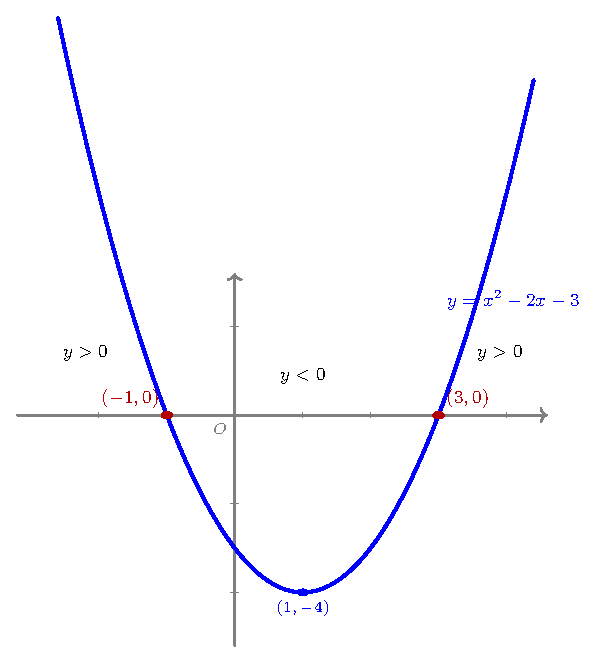
\includegraphics[width=0.56\textwidth]{parabola.pdf}
  \caption{$y=x^2-2x-3$ 的图象：交点、顶点与上下方}
\end{figure}

\subsection{二次函数与方程、不等式}

\key{探究三：判别式与求根公式}
对于方程 $ax^2+bx+c=0$（$a\neq0$），记 $\Delta=b^2-4ac$。
\begin{center}
\footnotesize
\setlength{\tabcolsep}{3pt}
\renewcommand{\arraystretch}{1.4}
\begin{tabular}{p{2.4cm}p{4.2cm}p{5.2cm}}
\toprule
$\Delta$ 的符号 & 方程的根 & 函数图象与 $x$ 轴的交点个数 \\
\midrule
$\Delta>0$ & 两个不相等的实数根 & 两个交点 \\
$\Delta=0$ & 两个相等的实数根 & 一个交点（相切） \\
$\Delta<0$ & 没有实数根 & 没有交点 \\
\bottomrule
\end{tabular}
\end{center}

当 $\Delta\geq0$ 时，求根公式：
\[
  x=\frac{-b\pm\sqrt{b^2-4ac}}{2a}.
\]

\key{探究四：三个二次的关系}
\begin{itemize}
  \item 令 $y=0$，得到一元二次方程，它的解就是函数图象与 $x$ 轴交点的横坐标；
  \item 令 $y>0$（或 $y<0$），得到一元二次不等式，它的解集就是函数图象在 $x$ 轴上方（或下方）部分所对应的 $x$ 的取值范围。
\end{itemize}

\key{一句话}：方程找交点，不等式找上下，根是边界。

\key{探究五：一元二次不等式}
\begin{example}
解不等式 $x^2-2x-3<0$。
\end{example}
\begin{solution}
方程 $x^2-2x-3=0$ 的两根为 $x_1=-1$，$x_2=3$。
因为 $a=1>0$，抛物线开口向上，在 $x$ 轴下方的部分是两根之间，
故解集为 $(-1,3)$。
\end{solution}

\begin{example}
解不等式 $-x^2+2x+3>0$。
\end{example}
\begin{solution}
两边同乘 $-1$，不等号方向改变，得 $x^2-2x-3<0$，解集为 $(-1,3)$。
\end{solution}

\key{口诀}：大于取两边，小于取中间（适用于 $a>0$ 的情形）。

\key{探究六：数轴穿根法}
对高次不等式，用数轴穿根法更快。它的关键是\key{先看最高次项系数的符号}：
系数为正从右上方起笔；系数为负就先两边同乘 $-1$（不等号方向改变），化为正。
\key{一律先化为正}，规则只有一条。

\begin{example}
解不等式 $(x+1)(x-2)(x-4)<0$。
\end{example}
\begin{solution}
最高次项系数为正。根为 $-1$、$2$、$4$。在数轴上标出后，从右上方起笔依次穿根，
得到各段符号依次为 $+$、$-$、$+$、$-$。
取小于 $0$ 的部分，解集为 $(-\infty,-1)\cup(2,4)$。
\end{solution}

\begin{figure}[htbp]
  \centering
  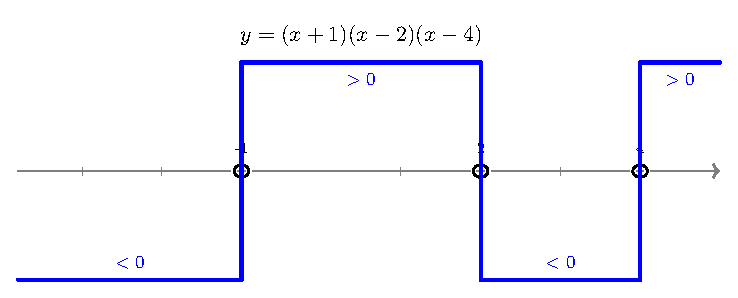
\includegraphics[width=0.70\textwidth]{ineq-on-axis.pdf}
  \caption{穿根折线与解集（空心点表示端点不取）}
\end{figure}

\key{步骤}：化标准形 $\to$ 求根标轴 $\to$ 右上起笔 $\to$ 奇穿偶不穿 $\to$ 取上下方 $\to$ 查端点。

\key{探究七：分式不等式}
分式不等式也用这条思路：先判断分子、分母的正负，再转化为整式不等式画图求解。
\[
  \frac{f(x)}{g(x)}>0 \iff f(x)g(x)>0 \quad (g(x)\neq0).
\]
\key{注意}：分母的零点取不到，必须画空心点。

\begin{example}
解不等式 $\dfrac{x+1}{x-2}\geq0$。
\end{example}
\begin{solution}
等价于 $(x+1)(x-2)\geq0$ 且 $x\neq2$。
根为 $-1$、$2$，从右上方起笔依次穿根，取大于等于 $0$ 的部分并去掉 $2$，
解集为 $(-\infty,-1]\cup(2,+\infty)$。
\end{solution}

\begin{figure}[htbp]
  \centering
  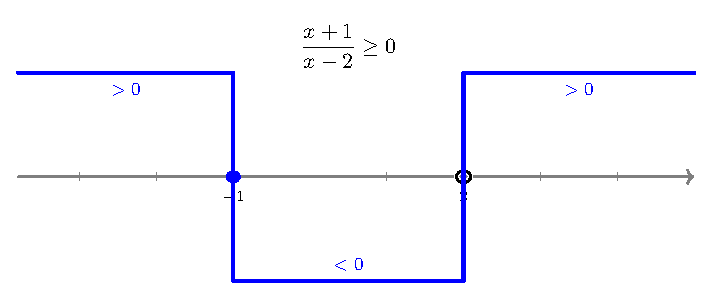
\includegraphics[width=0.70\textwidth]{rational-ineq.pdf}
  \caption{$\dfrac{x+1}{x-2}\geq0$：$-1$ 实心（可取），$2$ 空心（分母零点）}
\end{figure}

\key{探究八：解集在数轴上的表示}
穿根法是\key{求}解集的方法；本节是把已经求出的解集\key{画}出来。

\begin{figure}[htbp]
  \centering
  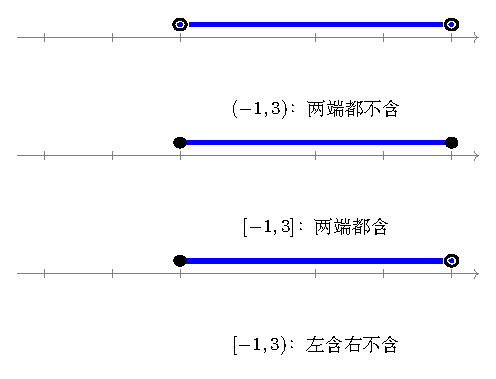
\includegraphics[width=0.56\textwidth]{interval-notation.pdf}
  \caption{区间在数轴上的三种端点情形}
\end{figure}

\key{约定}：空心圈表示不含该端点，实心点表示含有该端点。

\subsection{区间最值与恒成立}

\key{探究九：区间上的最值}
二次函数的最值只可能出现在顶点或区间端点处。
\begin{center}
\footnotesize
\setlength{\tabcolsep}{3pt}
\renewcommand{\arraystretch}{1.4}
\begin{tabular}{p{2.8cm}p{4.2cm}p{4.4cm}}
\toprule
对称轴 $x=h$ 的位置 & $a>0$ 的最小值 & $a>0$ 的最大值 \\
\midrule
$h<m$ & $f(m)$ & $f(n)$ \\
$m\leq h\leq n$ & $f(h)$（顶点） & 离对称轴较远的端点 \\
$h>n$ & $f(n)$ & $f(m)$ \\
\bottomrule
\end{tabular}
\end{center}

\key{开口向下时}（$a<0$）：上表的最小值与最大值\key{对调}——最小值落在上表最大值的位置，最大值落在上表最小值的位置。

\begin{problem}
求 $y=x^2-2x-3$ 在区间 $[0,4]$ 上的最大值与最小值。
\end{problem}
\begin{solution}
配方得 $y=(x-1)^2-4$，对称轴 $x=1\in[0,4]$。
$a=1>0$，故最小值在顶点处取得，为 $f(1)=-4$。
端点值 $f(0)=-3$，$f(4)=5$，故最大值为 $f(4)=5$。
\end{solution}

\begin{figure}[htbp]
  \centering
  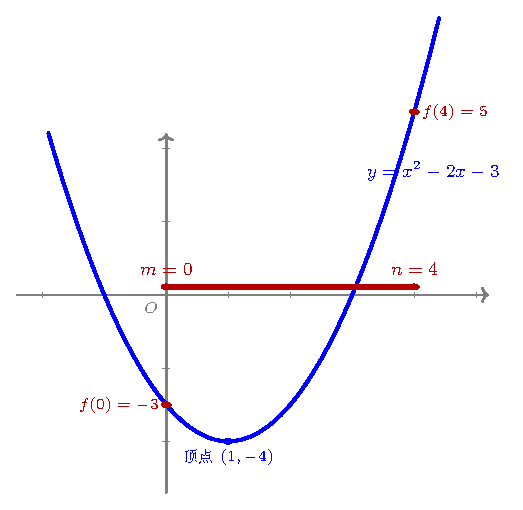
\includegraphics[width=0.60\textwidth]{interval-extreme.pdf}
  \caption{区间 $[0,4]$ 上的最值：顶点最小，端点最大}
\end{figure}

\begin{problem}
求 $y=x^2-2x-3$ 在区间 $[m,m+2]$ 上的最小值（$m$ 为参数）。
\end{problem}
\begin{solution}
对称轴 $x=1$。分三种情况：
\begin{itemize}
  \item 若 $1<m$，最小值为 $f(m)=m^2-2m-3$；
  \item 若 $m\leq1\leq m+2$，最小值为 $f(1)=-4$；
  \item 若 $1>m+2$，最小值为 $f(m+2)=m^2+2m-3$。
\end{itemize}
\end{solution}

\key{探究十：恒成立与能成立}
恒成立问题按「在什么范围上成立」分两类：在 $\mathbb{R}$ 上用判别式，在区间上化为最值。

\begin{problem}
若 $x^2+2x+c>0$ 对任意实数 $x$ 恒成立，求 $c$ 的取值范围。
\end{problem}
\begin{solution}
不等式恒成立，即函数 $y=x^2+2x+c$ 的图象全部在 $x$ 轴上方。
因为 $a=1>0$，只需判别式小于 $0$：
\[
  \Delta=4-4c<0\implies c>1.
\]
\end{solution}

\key{结论}：$a>0$ 且 $\Delta<0$（$>0$ 恒成立）；$a>0$ 且 $\Delta\leq0$（$\geq0$ 恒成立）。

\begin{problem}
若 $x^2-2x+m>0$ 对任意 $x\in[0,3]$ 恒成立，求 $m$ 的取值范围。
\end{problem}
\begin{solution}
设 $f(x)=x^2-2x+m$。恒成立即最小值大于 $0$。
对称轴 $x=1\in[0,3]$，故最小值为 $f(1)=m-1$，由 $m-1>0$ 得 $m>1$。
\end{solution}

\begin{problem}
若 $x^2-2x+m>0$ 对任意 $x\in[3,4]$ 恒成立，求 $m$ 的取值范围。
\end{problem}
\begin{solution}
对称轴 $x=1<3$，函数在 $[3,4]$ 上递增，
最小值为 $f(3)=m+3$，由 $m+3>0$ 得 $m>-3$。
\end{solution}

\key{注意}：在区间上恒成立不能套判别式。
上例若套 $\Delta<0$，得 $m>1$，会漏掉 $(-3,1]$ 一整段。

\key{对偶}：\key{能成立}（存在 $x$ 使 $f(x)>0$）看最大值——
存在 $x\in[a,b]$ 使 $f(x)>0$ $\iff$ $f$ 在 $[a,b]$ 上的最大值 $>0$。
恒成立看最小值，能成立看最大值，方向相反。

\key{另解（分离参数）}：$x^2-2x+m>0$ 在 $[a,b]$ 上恒成立
$\iff m>-x^2+2x$ 在 $[a,b]$ 上恒成立 $\iff m$ 大于右边在 $[a,b]$ 上的最大值。

\end{explore}

\begin{inclasstest}
\begin{enumerate}
  \item 把 $y=3x^2-6x+2$ 配方成顶点式；
  \item 求 $y=-x^2+2x+1$ 的顶点、对称轴与最值；
  \item 解不等式 $x^2-5x+6>0$；
  \item 解不等式 $x^2-4x+4\leq0$；
  \item 用数轴穿根法解不等式 $(x-1)(x-2)(x-3)\geq0$；
  \item 解不等式 $\dfrac{x-1}{x+2}<0$，并把解集画在数轴上；
  \item 求 $y=x^2-2x-3$ 在区间 $[0,4]$ 上的最大值与最小值；
  \item 若 $x^2-2x+m>0$ 对任意 $x\in[3,4]$ 恒成立，求 $m$ 的取值范围。
\end{enumerate}
\end{inclasstest}

\begin{afterclass}
\begin{enumerate}
  \item 求 $y=-2x^2+4x-3$ 的顶点、对称轴与最值；
  \item 解不等式 $x^2-3x-4\geq0$；
  \item 解不等式 $-2x^2+4x-3>0$；
  \item 用数轴穿根法解不等式 $(x+2)(x-1)(x-3)<0$；
  \item 解不等式 $\dfrac{2x-1}{x-3}\geq1$；
  \item 求 $y=2x^2-4x+1$ 在 $[-1,2]$ 上的最大值与最小值；
  \item 若 $x^2+ax+1>0$ 对任意实数 $x$ 恒成立，求 $a$ 的取值范围；
  \item 若存在 $x\in[0,2]$，使 $x^2-2x+m>0$，求 $m$ 的取值范围；
  \item 默写一张解题流程图。
\end{enumerate}
\end{afterclass}
